% !TEX root = ../../../main.tex
% 来源：中学数学实验教材·第三册（高中数学）
% 章节：函数及其图象 / 函数及其图象
% 原始文件：4.tex，行 856-868
% 类型：tikz
% ---
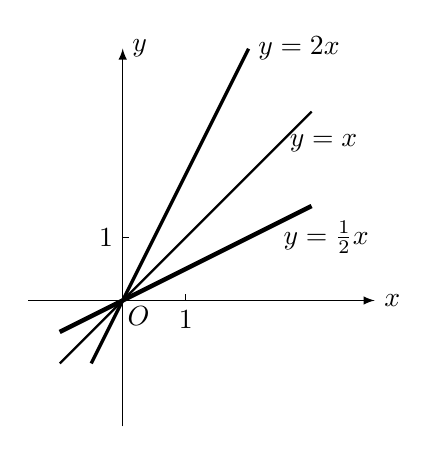
\begin{tikzpicture}[>=latex, scale=.8]
    \draw[->](-1.5,0)--(4,0)node[right]{$x$};
    \draw[->] (0,-2)--(0,4)node[right]{$y$};
\draw [thick, domain=-1:3, samples=100] plot(\x, {\x});
\draw [very thick, domain=-.5:2, samples=100] plot(\x, {2*\x});
\draw [ultra thick, domain=-1:3, samples=100] plot(\x, {0.5*\x});
\draw (1,0)node[below]{1}--(1,.1);
\draw (0,1)node[left]{1}--(.1,1);
\node at (2,4) [right]{$y=2x$};
\node at (2.5,2.5) [right]{$y=x$};
\node at (2.4,1) [right]{$y=\frac{1}{2}x$};
\node at (.25,-.25){$O$};
\end{tikzpicture}
